\section{Threat Model}\label{sec:threatModel}
We assume that APT attacks launch attacks with the following features:

\begin{itemize}[leftmargin=*]
    \item \textbf{Stealthy}. The attacker employs covert tactics, concealing their malicious activities amid a substantial volume of benign background data, resulting in the victim system exhibiting behavior akin to a benign mode.
    \item \textbf{Evolving}. Professional attacker groups continually innovate, extending their targets to a broader array of system processes and adeptly adjusting to the latest defensive mechanisms to maintain a competitive edge.
    %As professional attacker groups continue to innovate, they are targeting an ever-expanding range of system processes and adapting to the latest defensive measures in order to stay ahead of the game.
    \item \textbf{Frequent usage of zero-day exploits}. The attacker primarily relies on zero-day exploits, resulting in a lack of advanced knowledge w.r.t. the specific attack patterns.
\end{itemize}

\section{Methodology of \tool}

\begin{figure*}[ht]
    \centering
      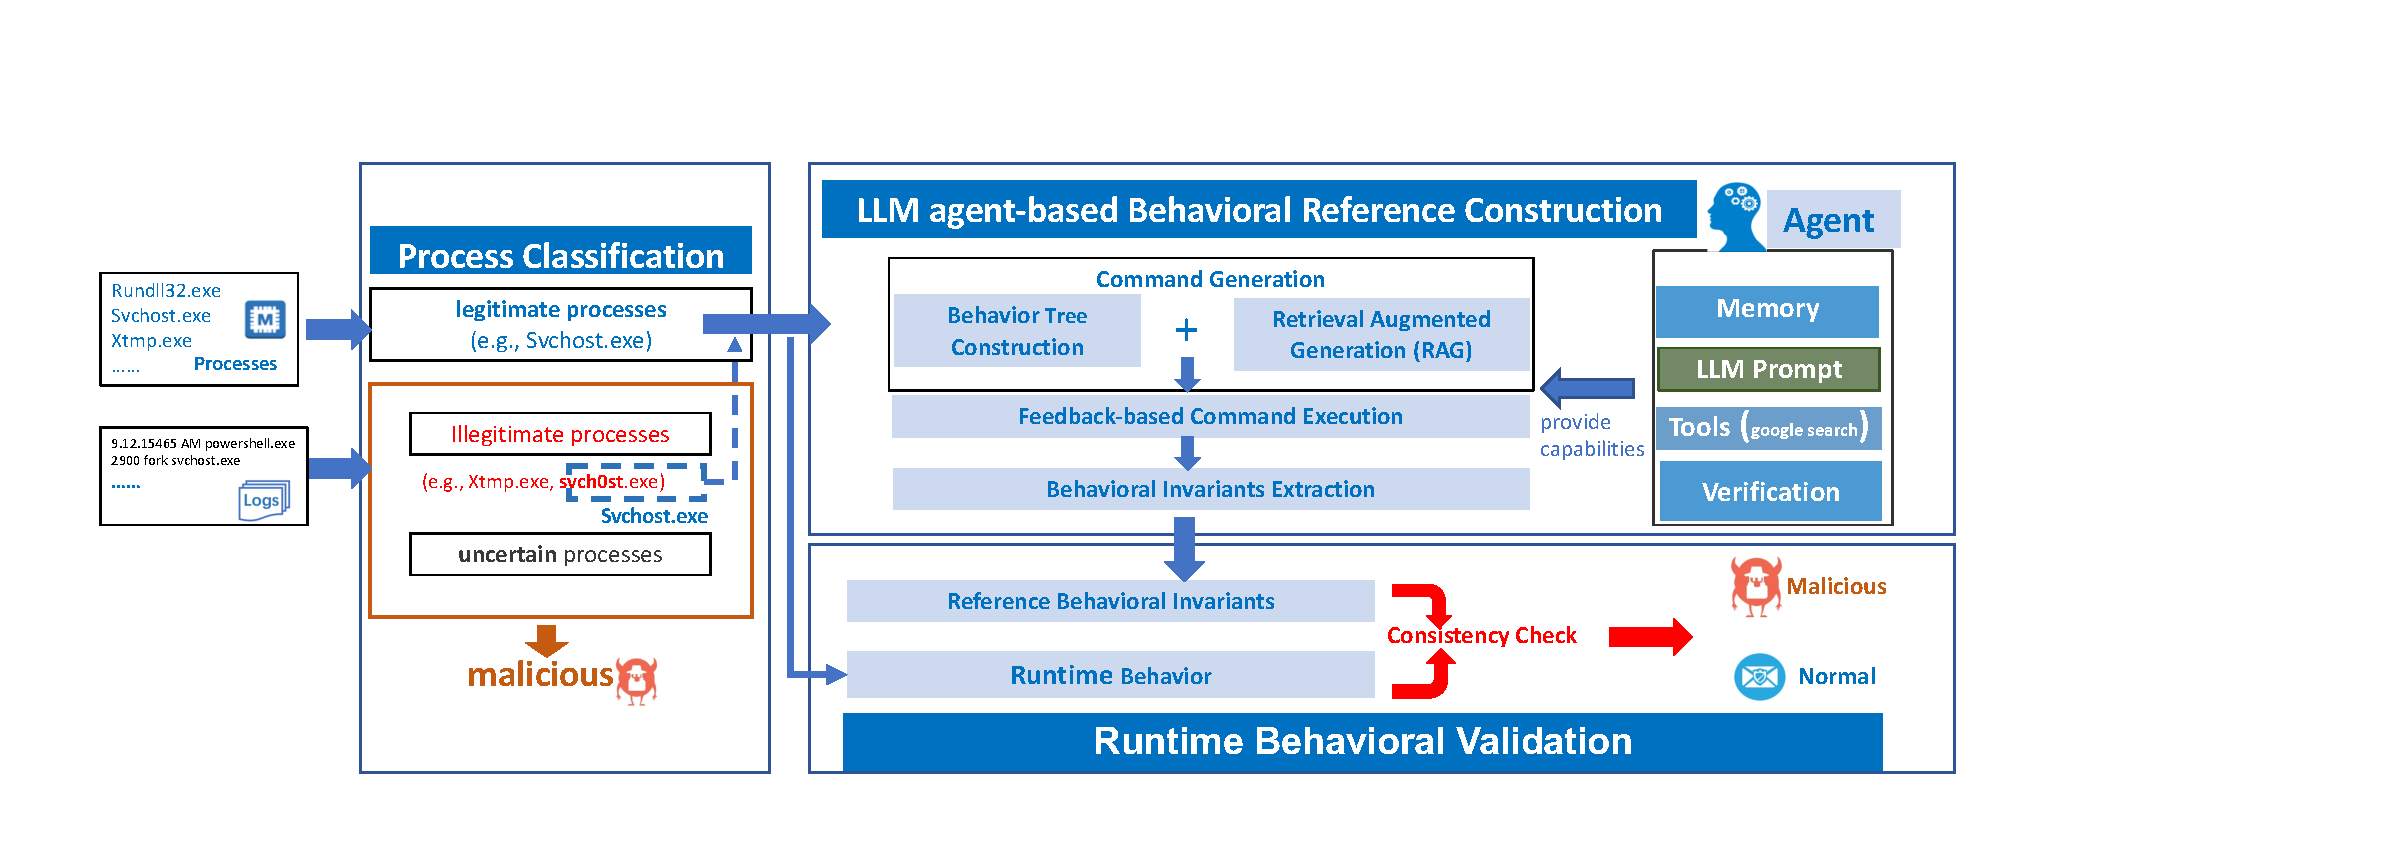
\includegraphics[width=0.85\textwidth]{figs/framework_new2.pdf}
      % \caption{An overview of \tool.}
    \caption{An overview of \tool. }
    %Given a bundle of logs collected from system processes, \tool first filters legitimate processes as detection targets while regarding the others as potential malicious attacks. Then, \tool constructs a behavioral invariant for each legitimate process via the Behavioral Reference Construction Module, which is in the form of disjunction and/or conjunction of reference propositions. Finally, the Runtime Behavioral Validation module will transform both the behavioral invariants generated before and the original runtime systems logs into sets of logical propositions for the target processes, respectively. By checking the consistency of two sets of propositions (e.g., checking the satisfiability of the conjunction of all propositions from the two sets), \tool will return the detection result.}
    \label{fig-framework}
\end{figure*}


\subsection{Technical Challenges}\label{sec:challenges}
A straightforward idea is to utilize the knowledge extraction capabilities in LLMs to facilitate the construction of more comprehensive behavioral invariants for victim system processes first, which can then be employed for conducting further thorough attack detection analysis. Recall that,
when dealing with the evolution of attacks or their stealthy tactics, supplemental knowledge can be very crucial. Moreover, in contrast to learning-based detection methods, this approach obviates the requirement for pre-defined attack patterns, which also enhances its adaptability and versatility in addressing evolving threat landscapes.
However, the direct employment of LLMs in our setting gives rise to the following three notable technical challenges:

\noindent
{\bf CH-\circled{1} Context Dependency.} %  :
LLMs' ability to extract process behavior knowledge heavily relies on the context provided in the input. Without sufficient context or in cases of ambiguous information, LLMs struggle to generate rich and accurate behavior descriptions. This limitation is significant in complex domains where behaviors are intricately linked to specific circumstances or prerequisites.

\noindent
{\bf CH-\circled{2} Provision of Outdated Information.} % \circled{2}
The dynamic nature of knowledge means that documentation and processes are regularly updated. However, LLMs might not be immediately updated to reflect these changes, leading to the provision of information that is outdated and potentially misleading.

\noindent
{\bf CH-\circled{3} Hallucination Issues.} % \circled{3}
Hallucination in LLMs refers to the generation of information that is not based on the input data or grounded in reality. This includes providing false information in the absence of clear answers and creating responses based on non-authoritative or unreliable sources.


\subsection{Overview of \tool}
In this work, we propose an effective LLMs-based APT attack detection framework, named \tool, addressing all the above challenges. The overview of \tool can be found in Figure~\ref{fig-framework}.

\tool comprises three main modules: Process Classification, Behavioral Invariants Construction, and Runtime Behavioral Validation. Given a bundle of logs collected from system processes, \tool first filters legitimate processes as detection targets while regarding the others as potential malicious attacks. Then, the Behavioral Reference Construction Module constructs a behavioral invariant for each authorized process, specifically utilizing a structure composed of facts and temporal behavioral invariant. Finally, the Runtime Behavioral Validation module transforms both the previously generated behavioral invariants and the original runtime system logs into a logical framework for the target processes, respectively. By evaluating the consistency between the reference and runtime invariants, the tool determines the detection outcome, where consistency indicates normal behavior and inconsistency signifies malicious activity.

Specifically, to address the technical challenges outlined in Section~\ref{sec:challenges}, We employ the LLM agent architecture to fully harness the capabilities of both LLMs and traditional software for constructing the Behavioral Reference as shown in Figure~\ref{fig-framework}.


\noindent
{\bf Process Behavior Tree Construction.} To provide an enriched contextual environment for LLMs, we first capture a comprehensive range of behaviors for each process, i.e., creating a behavior tree for each process. Then, the Large Language Models (LLM) continuously expands its knowledge of this behavior tree through a ``self-ask'' manner. Finally, the LLM benefits greatly from this behavior tree as it provides an enriched contextual environment, which can greatly tackle {\bf CH-\circled{1}}.

\noindent
{\bf Retrieval Augmented Generation.} 
To address challenges related to outdated information and the reliability of knowledge, we employ a Retrieval Augmented Generation (RAG) module. This module initially conducts a Google search to obtain the top $N$ documents relevant to the topic at hand. It then utilizes these documents to construct additional commands. These newly generated commands are integrated with those produced in the initial step, facilitating the acquisition of more current and authoritative knowledge. This approach primarily aims to overcome the {\bf CH-\circled{2}} and {\bf CH-\circled{3}} by ensuring the information provided is both up-to-date and credible.


\noindent
{\bf Feedback-based Command Execution.} 
Our third step involves executing the commands generated in the first two steps within the system. To address {\bf CH-\circled{3}}, we implement a feedback execution update mechanism. Initially, if the commands encounter execution challenges such as missing parameters, files, or parameter dependencies, these issues are directly fed back to the LLM, which then updates the current commands accordingly. Following the execution, actual logs are obtained, which are used for subsequent steps. This method ensures that execution hurdles are promptly identified and rectified, leading to a more efficient and error-free operation.

\noindent
{\bf Behavioral Invariants Extraction.} In the final step, we first employ common term and prefix-span sequence mining algorithm to unearth deeper relationships within the logs. Subsequently, LLMs are utilized to interpret these invariants, providing insights into the underlying patterns and associations. This integrated approach not only maximizes the strengths of both methodologies but also facilitates a comprehensive analysis of the logs, leading to a richer understanding of the data.






